\section{Langkah-Langkah Percobaan}
VPN
\begin{enumerate}
	\item Reset konfigurasi router
	\item Login ke router di winbox
	\item konfigurasi DHCP \\
	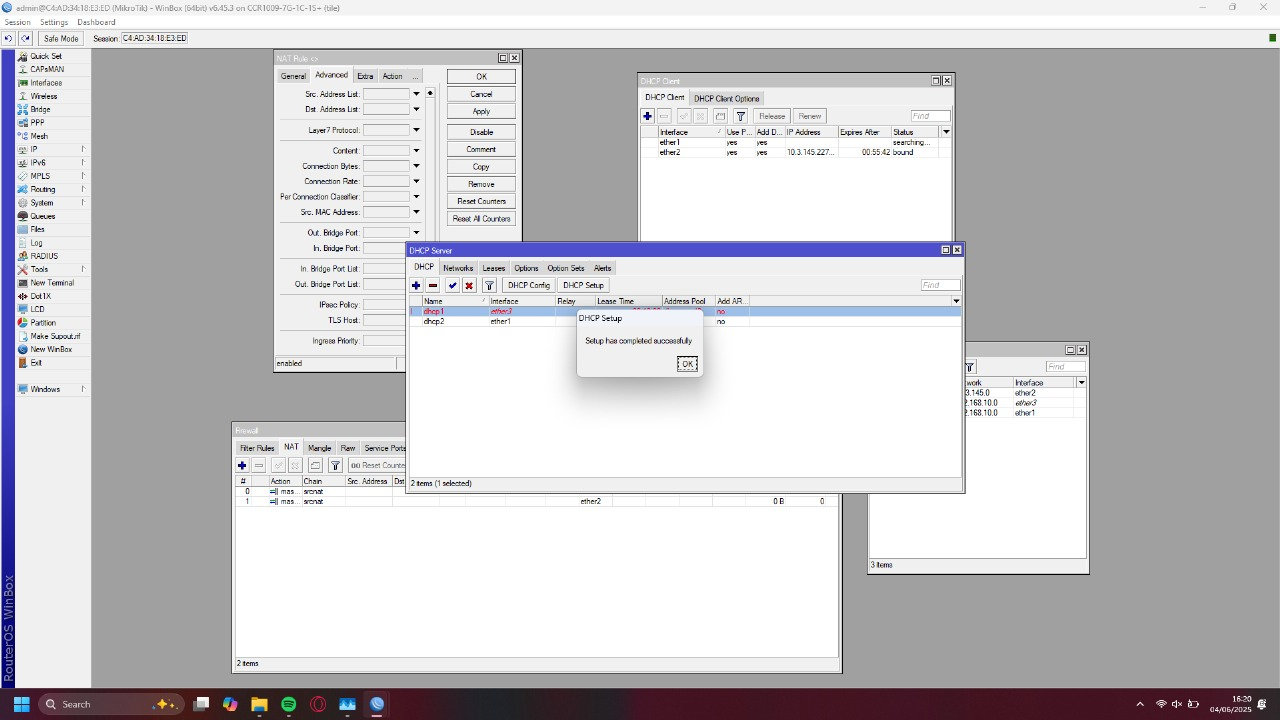
\includegraphics[width=0.7\textwidth]{P5/img/dhcp.jpg}
	\item konfigurasi Firewall NAT\\
	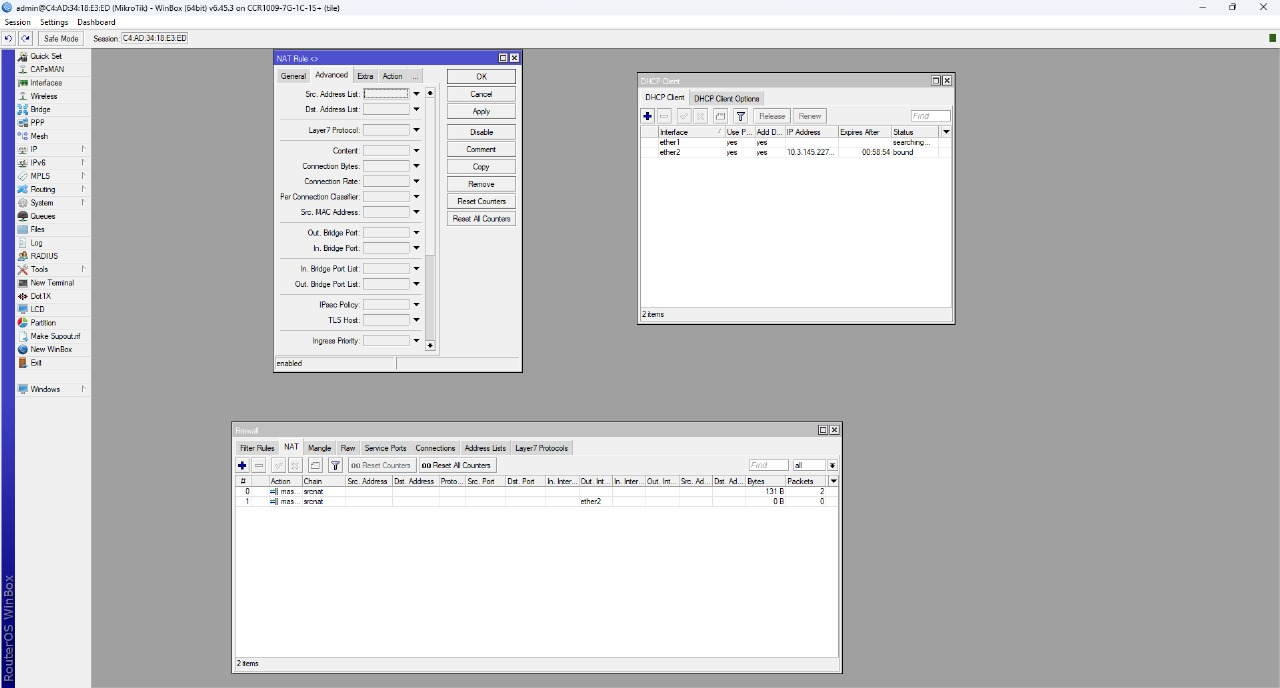
\includegraphics[width=0.7\textwidth]{P5/img/firewall.jpg}
	\item konfigurasi Alamat IP lokal LAN \\
	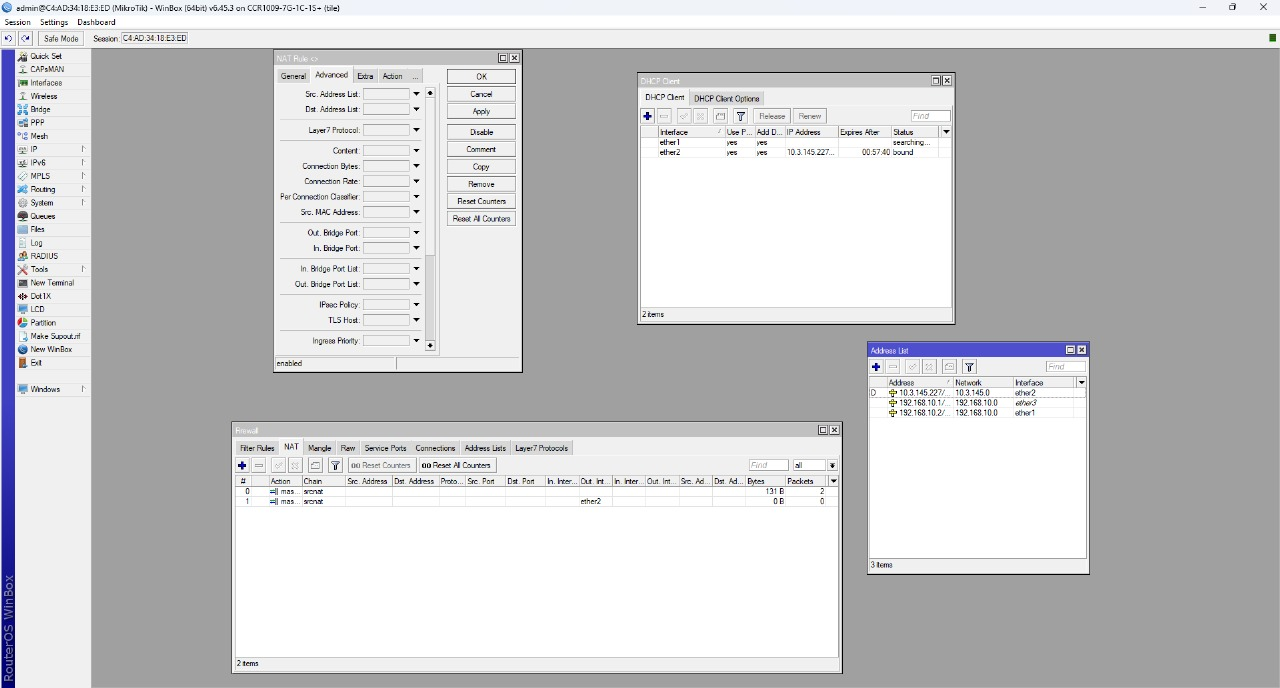
\includegraphics[width=0.7\textwidth]{P5/img/ip1.jpg}
	\item konfigurasi DHCP server untuk memberikan alamat IP kepada PC2 yang akan terhubung dengan VPN\\
	\item Ubah pengaturan untuk ether1 di menu \texttt{interface} ke proxy ARP\\
	\item Aktifkan PPTP Server\\
	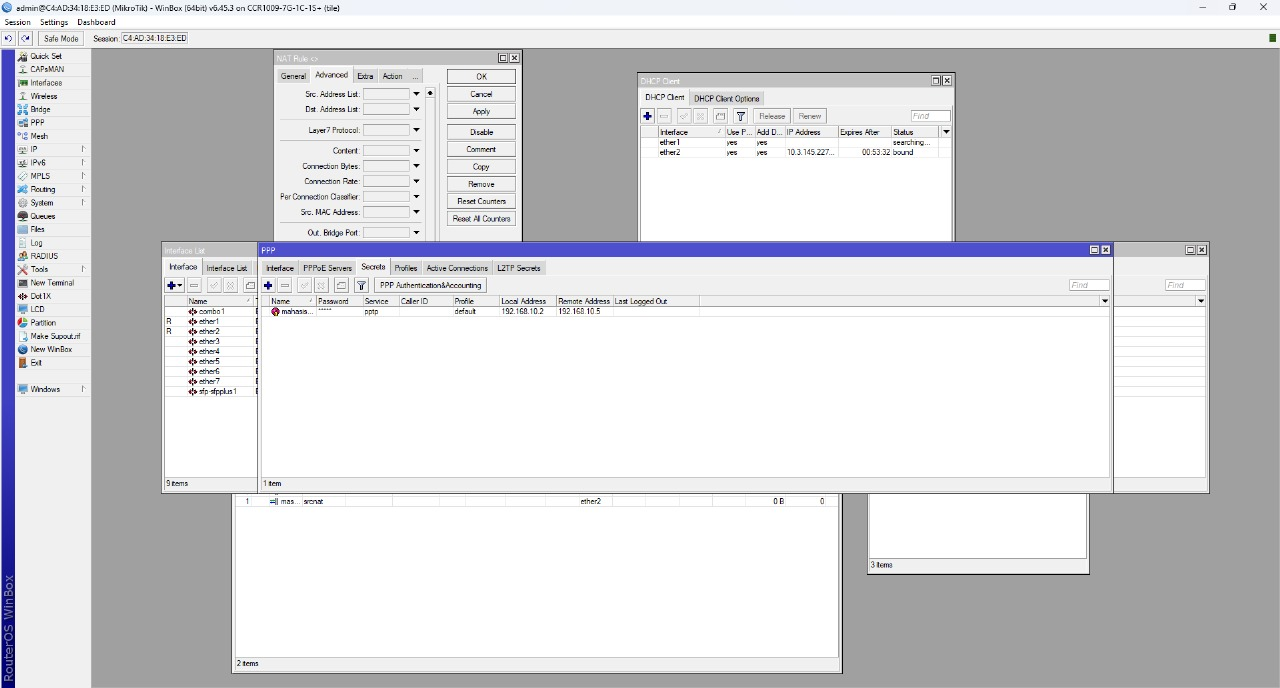
\includegraphics[width=0.7\textwidth]{P5/img/ptpn.jpg}
	\item Buat username dan password yang akan digunakan untuk login ke VPN\\
	\item Hubungkan PC2 ke VPN di settings\\
	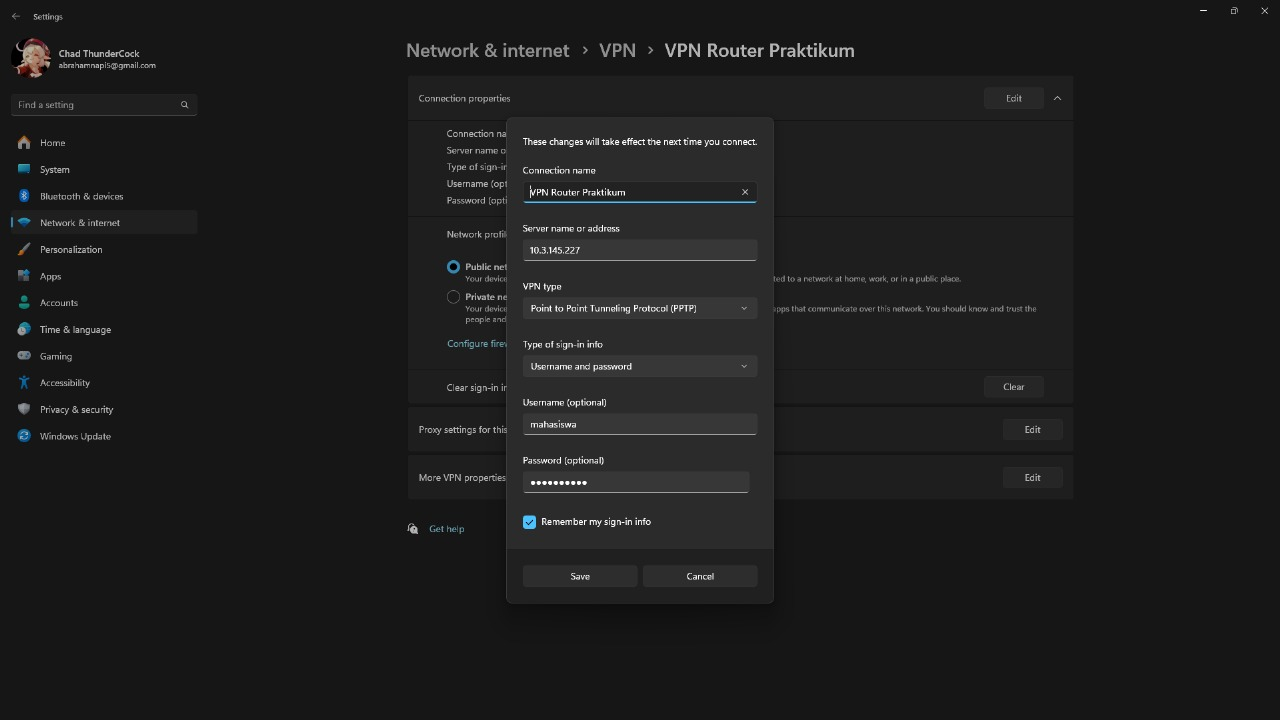
\includegraphics[width=0.7\textwidth]{P5/img/vpn.jpg}
	\item cek alamat IP di PC2 dengan menggunakan \texttt{ipconfig}\\
	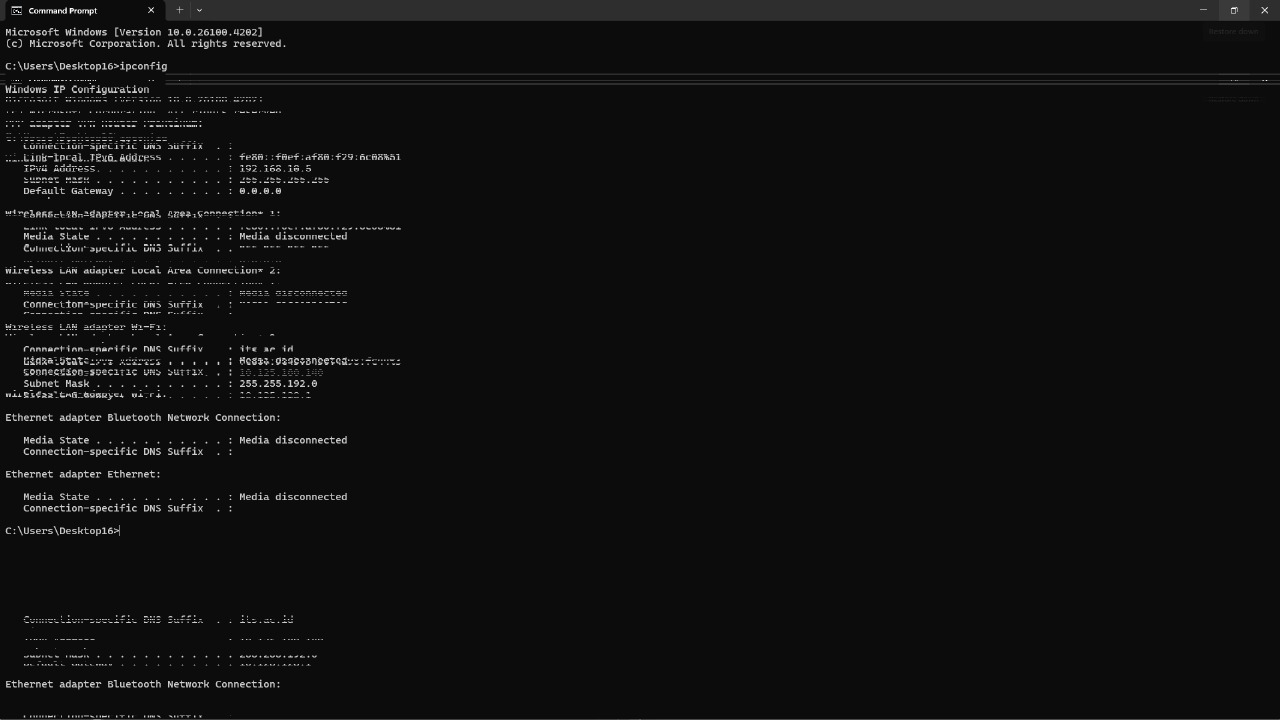
\includegraphics[width=0.7\textwidth]{P5/img/ipconfig.jpg}
	\item ping router dari PC2\\
	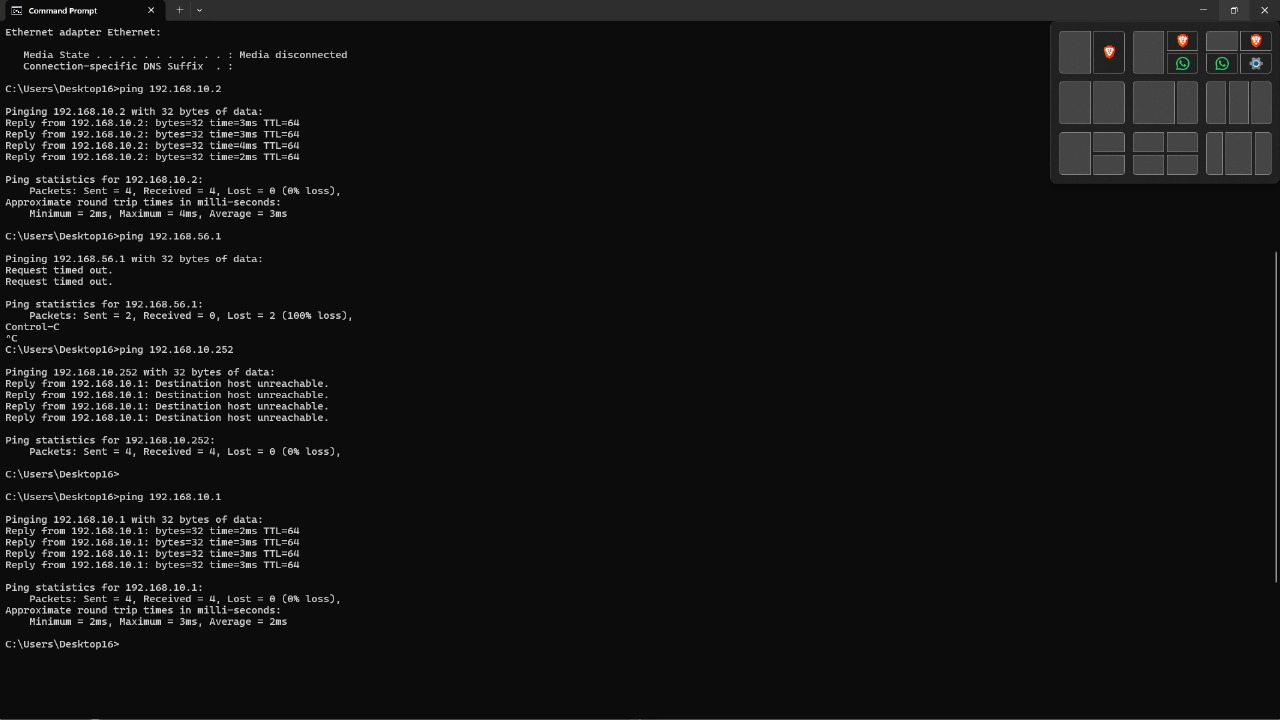
\includegraphics[width=0.7\textwidth]{P5/img/ping3.jpg}
\end{enumerate}
QoS
\begin{enumerate}
	\item Buka menu Queues dan buat aturan baru\\
	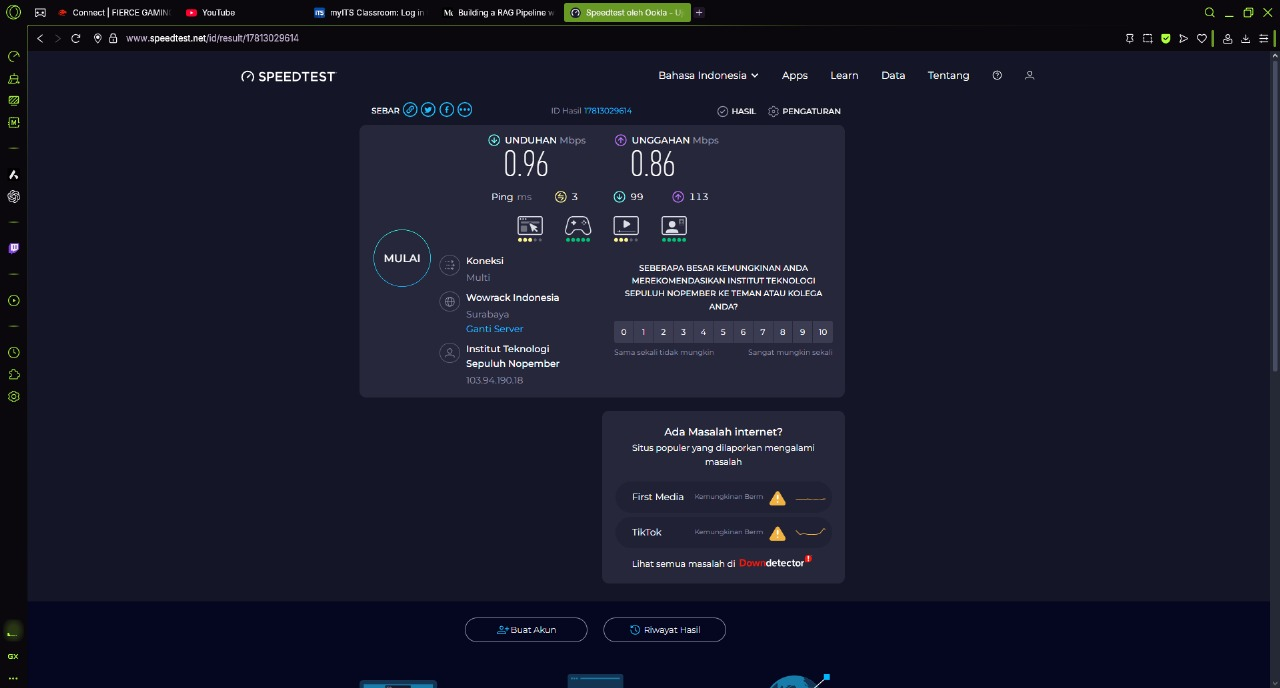
\includegraphics[width=0.7\textwidth]{P5/img/queue.jpg}
	\item Atur batas(limit) untuk upload dan download\\
	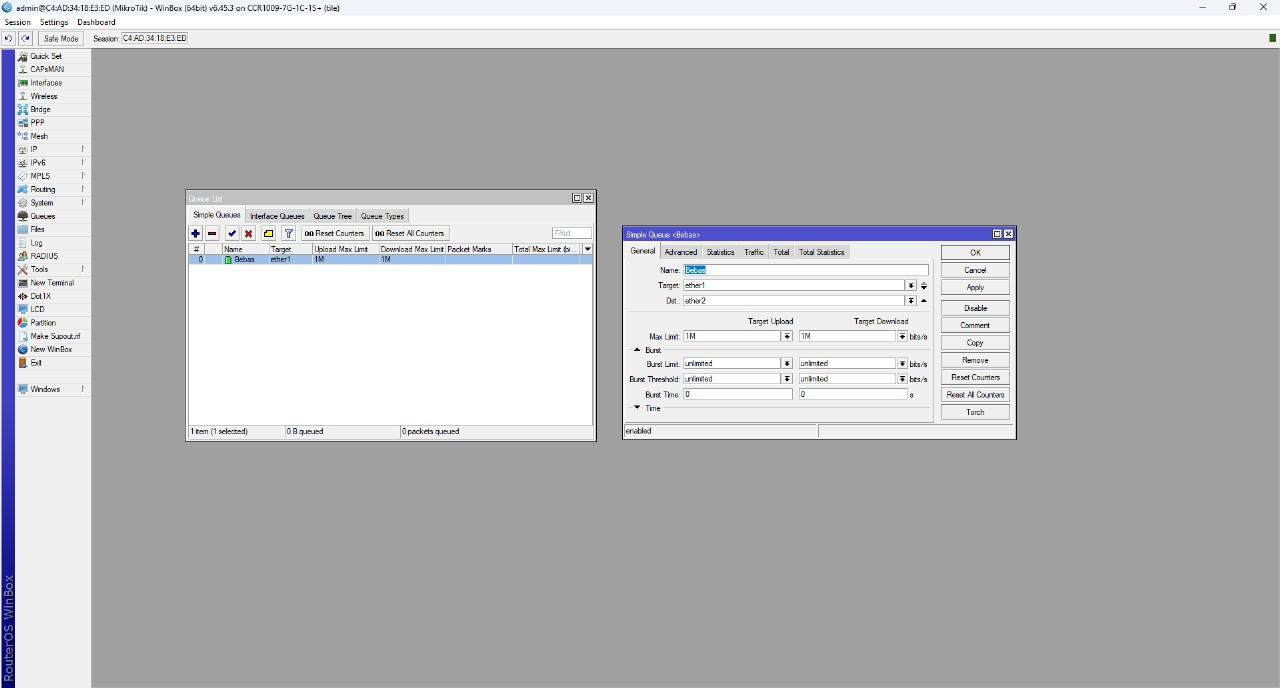
\includegraphics[width=0.7\textwidth]{P5/img/setqueue.jpg}
	\item cek traffic saat queue\\
	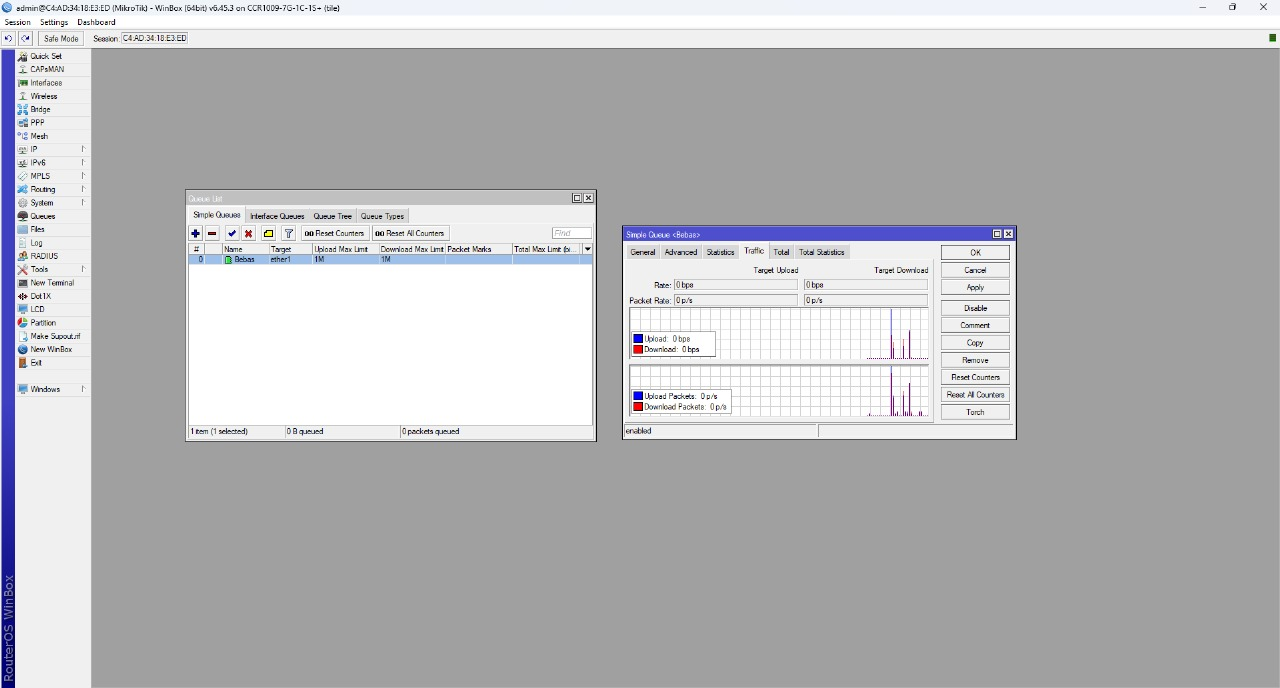
\includegraphics[width=0.7\textwidth]{P5/img/traffic.jpg}
	\item matikan queue dan lihat kembali
	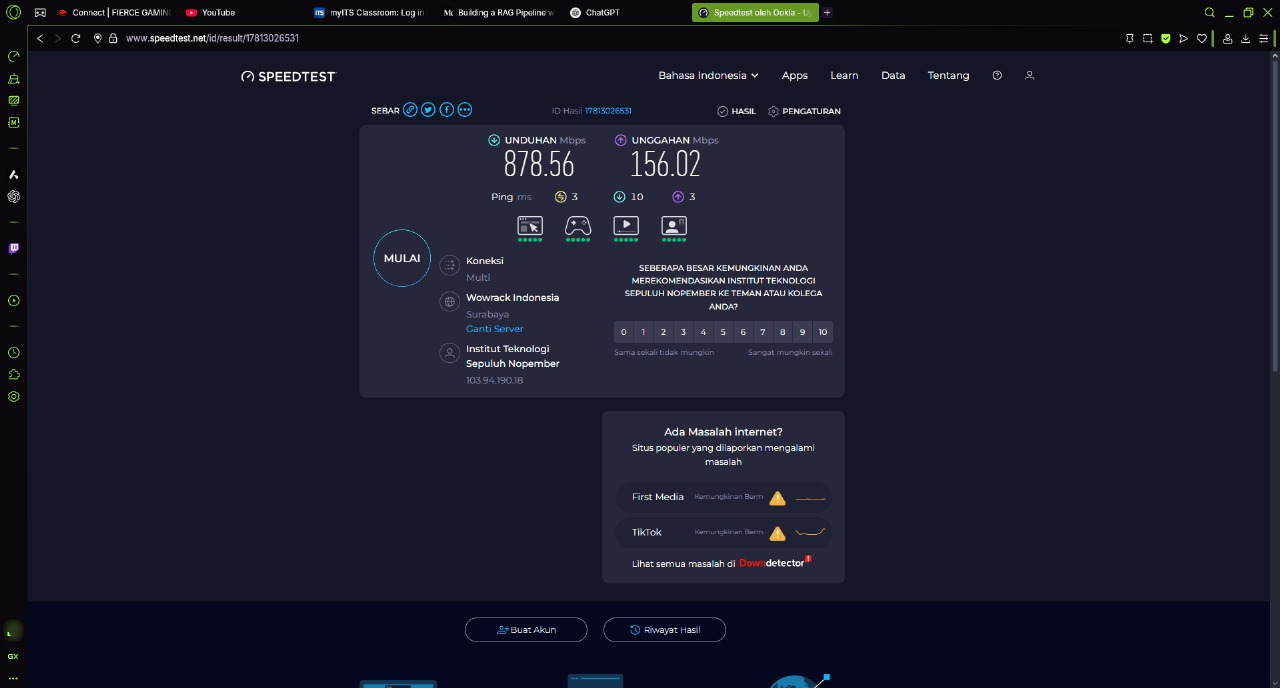
\includegraphics[width=0.7\textwidth]{P5/img/noqueue.jpg}
	
\end{enumerate}

\section{Analisis Hasil Percobaan}
Berdasarkan dua skenario praktikum yang telah saya lakukan pada router MikroTik, saya dapat menganalisis fungsionalitas dan relevansi dari setiap konfigurasi yang diterapkan.

\subsection*{$\bullet$ Analisis Konfigurasi VPN PPTP}
\addcontentsline{toc}{subsection}{Analisis Konfigurasi VPN PPTP}
Pada skenario pertama, saya berhasil membangun sebuah server VPN untuk koneksi \textit{remote access}. Proses ini menunjukkan beberapa poin penting. Pengaktifan \textbf{PPTP Server} pada router berfungsi sebagai "pendengar" yang siap menerima koneksi dari klien. Pembuatan kredensial pada tab \textbf{Secrets} adalah inti dari keamanan akses, di mana saya mendefinisikan username, password, serta alokasi alamat IP untuk klien yang akan terhubung.
Keberhasilan ping dari laptop klien (yang mendapat IP \texttt{192.168.10.5}) ke gateway router (\texttt{192.168.10.2}) dan ke PC lain di LAN membuktikan bahwa "terowongan" virtual telah terbentuk. Paket data dari laptop saya dibungkus menggunakan protokol PPTP, dikirim melalui internet, lalu dibuka kembali oleh router dan diteruskan ke jaringan lokal. Penggunaan \textbf{proxy-arp} pada antarmuka LAN juga krusial, karena memungkinkan router untuk "mewakili" klien VPN dalam komunikasi di jaringan lokal, sehingga seolah-olah klien VPN tersebut berada di segmen jaringan yang sama.

\subsection*{$\bullet$ Analisis Konfigurasi QoS dengan Simple Queue}
\addcontentsline{toc}{subsection}{Analisis Konfigurasi QoS dengan Simple Queue}
Pada skenario kedua, saya mengimplementasikan Quality of Service (QoS) untuk membatasi bandwidth. Saya menyimpulkan bahwa \textbf{Simple Queue} adalah metode yang sangat efektif dan mudah untuk manajemen bandwidth skala kecil hingga menengah. Dengan menargetkan seluruh subnet LAN (\texttt{192.168.10.0/24}), saya dapat menerapkan satu aturan untuk semua klien yang terhubung.
Pengaturan \textbf{Max Limit} ke \texttt{1M} terbukti berhasil membatasi kecepatan unduh dan unggah klien di sekitar 1 Mbps, seperti yang ditunjukkan oleh hasil perbandingan \textit{speed test}. Hal ini menunjukkan bahwa Simple Queue bekerja dengan cara memberlakukan batas atas (hard limit) pada lalu lintas yang cocok dengan target yang ditentukan. Fitur ini sangat relevan untuk lingkungan seperti jaringan kantor kecil atau publik di mana alokasi bandwidth yang adil dan terkontrol sangat diperlukan untuk menjaga stabilitas jaringan.


\section{Hasil Tugas Modul}
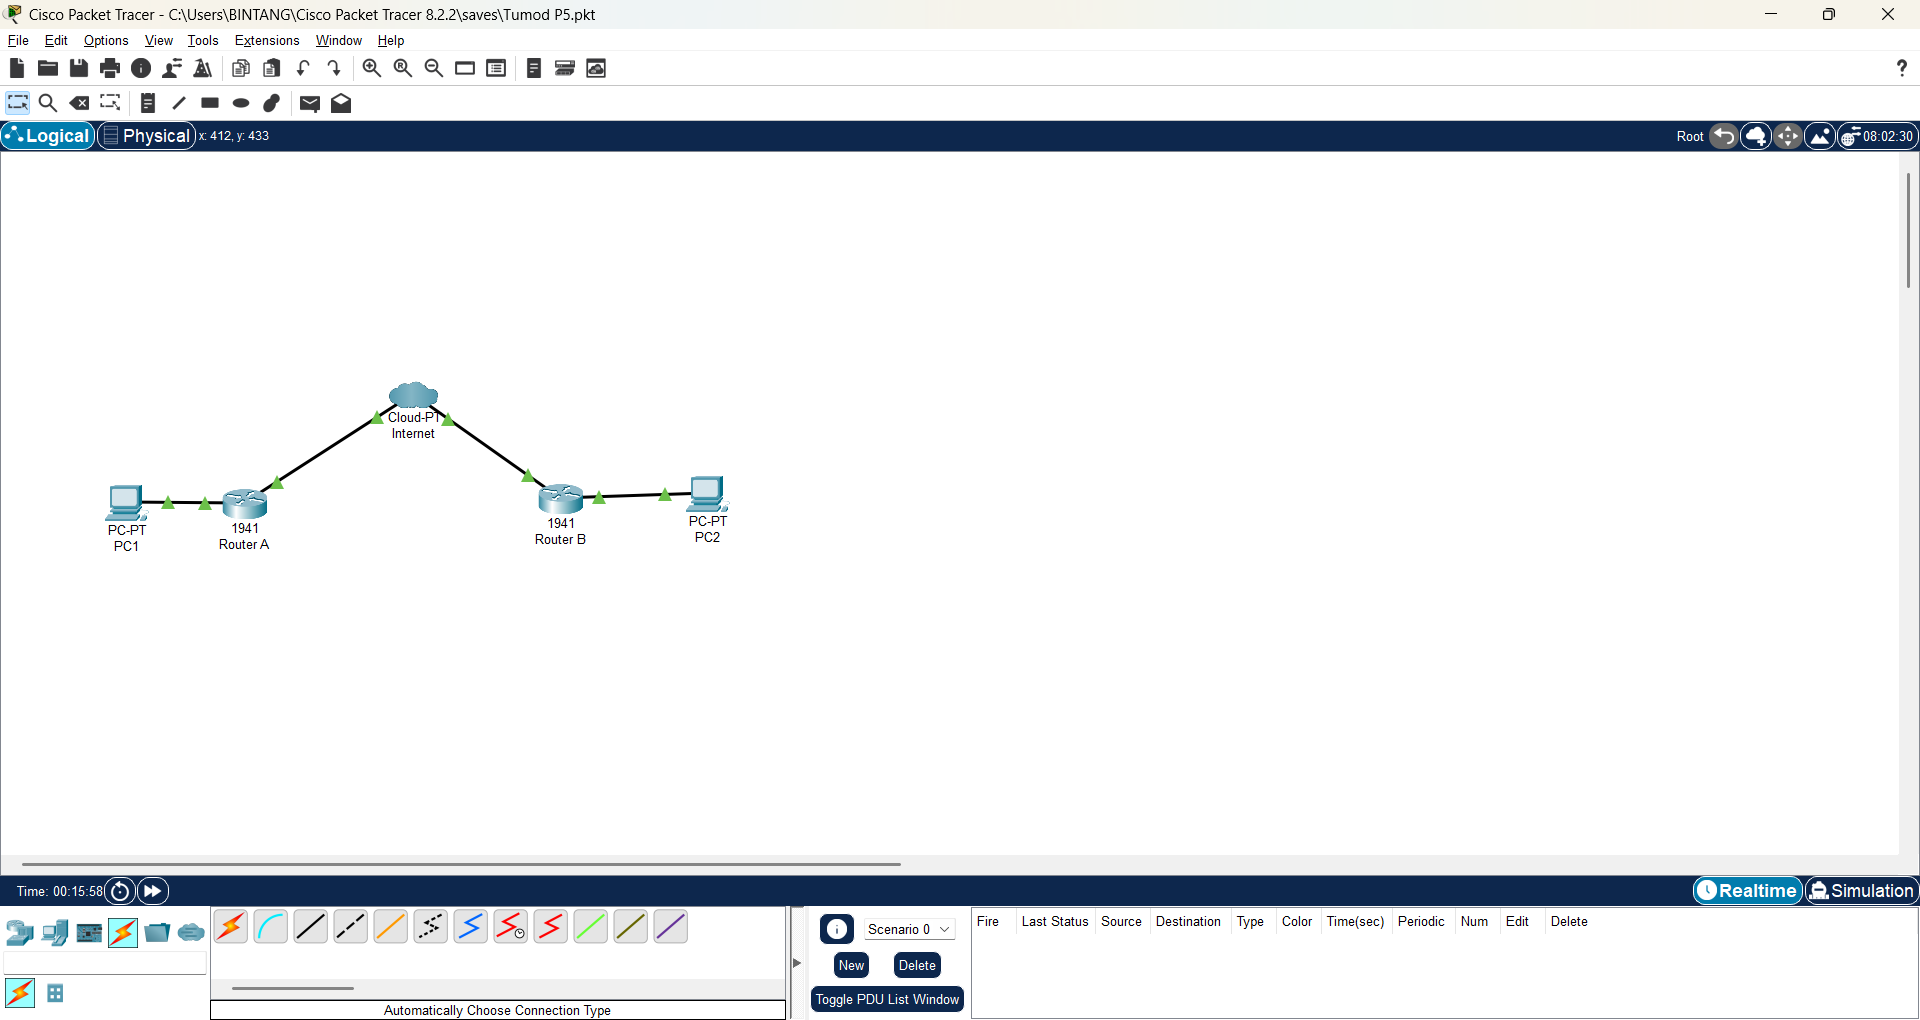
\includegraphics[width=0.7\textwidth]{P5/img/topologi.png}
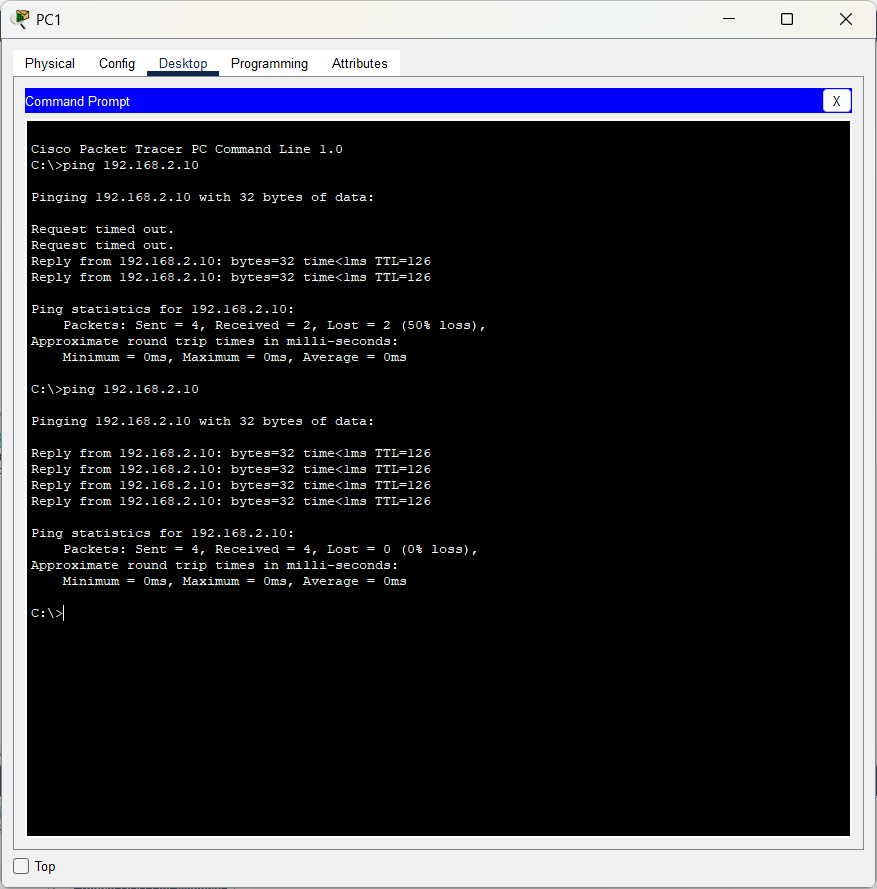
\includegraphics[width=0.7\textwidth]{P5/img/ping1.png}
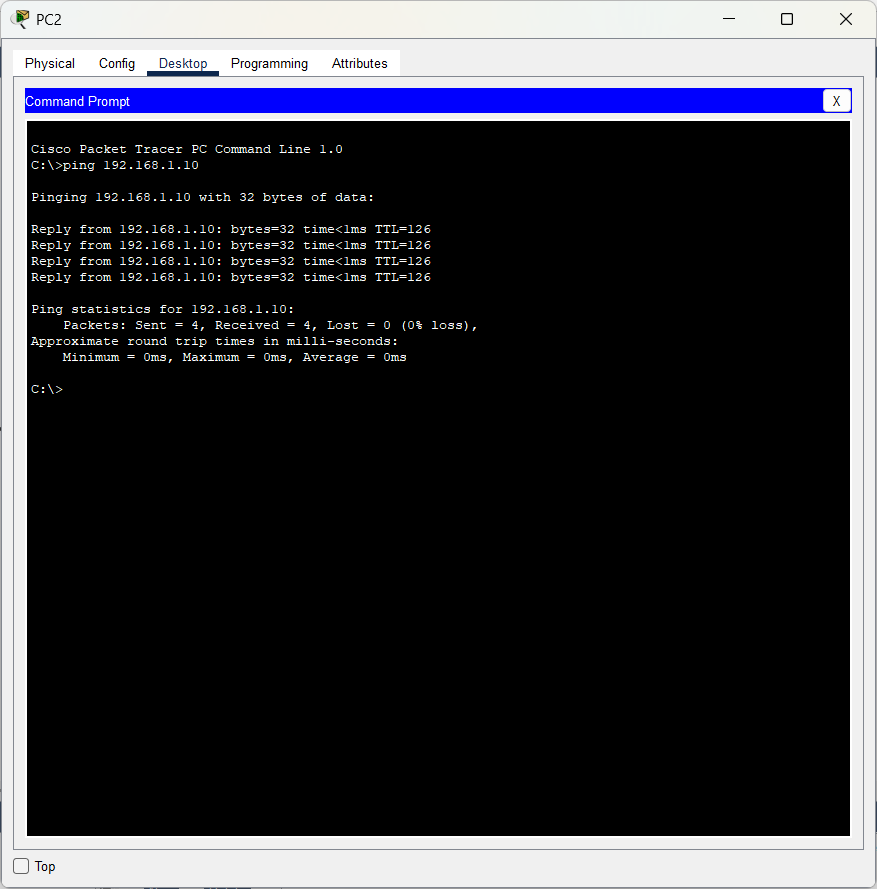
\includegraphics[width=0.7\textwidth]{P5/img/ping2.png}

Berdasarkan hasil simulasi telah berhasil dilakukan ping antar PC

\section{Kesimpulan}
Praktikum modul kelima ini memberikan pemahaman yang utuh mengenai teknologi tunneling dan manajemen lalu lintas jaringan. Dari materi teori, saya memahami berbagai jenis protokol tunneling, dengan IPSec sebagai standar keamanan tinggi dan GRE sebagai metode enkapsulasi yang fleksibel. Pada praktikum MikroTik, saya berhasil menerapkan konsep ini secara nyata dengan membangun server VPN PPTP untuk skenario \textit{remote access}, yang membuktikan bagaimana sebuah "terowongan" logis dapat menghubungkan klien eksternal ke jaringan internal dengan aman. Selain itu, implementasi \textit{Simple Queue} memberikan pengalaman langsung dalam melakukan manajemen bandwidth, sebuah aspek krusial dari Quality of Service (QoS) untuk menjaga performa jaringan.

Selanjutnya, pada Tugas Modul, saya mengintegrasikan pengetahuan ini dalam skala yang berbeda melalui simulasi \textit{site-to-site tunnel}. Penggunaan GRE tunnel di Cisco Packet Tracer secara efektif mendemonstrasikan bagaimana dua jaringan privat yang terpisah dapat disatukan melalui jaringan publik. Proses ini menegaskan pentingnya routing berlapis: routing di jaringan fisik (dasar) untuk membentuk tunnel, dan routing di atas tunnel (overlay) untuk melewatkan data pengguna. Secara keseluruhan, saya menyimpulkan bahwa teknologi tunneling dan QoS adalah pilar fundamental dalam rekayasa jaringan modern, yang masing-masing berfungsi untuk menyediakan konektivitas yang aman dan terukur melintasi batas-batas jaringan fisik.

\section{Lampiran}
\subsection{Dokumentasi saat praktikum}
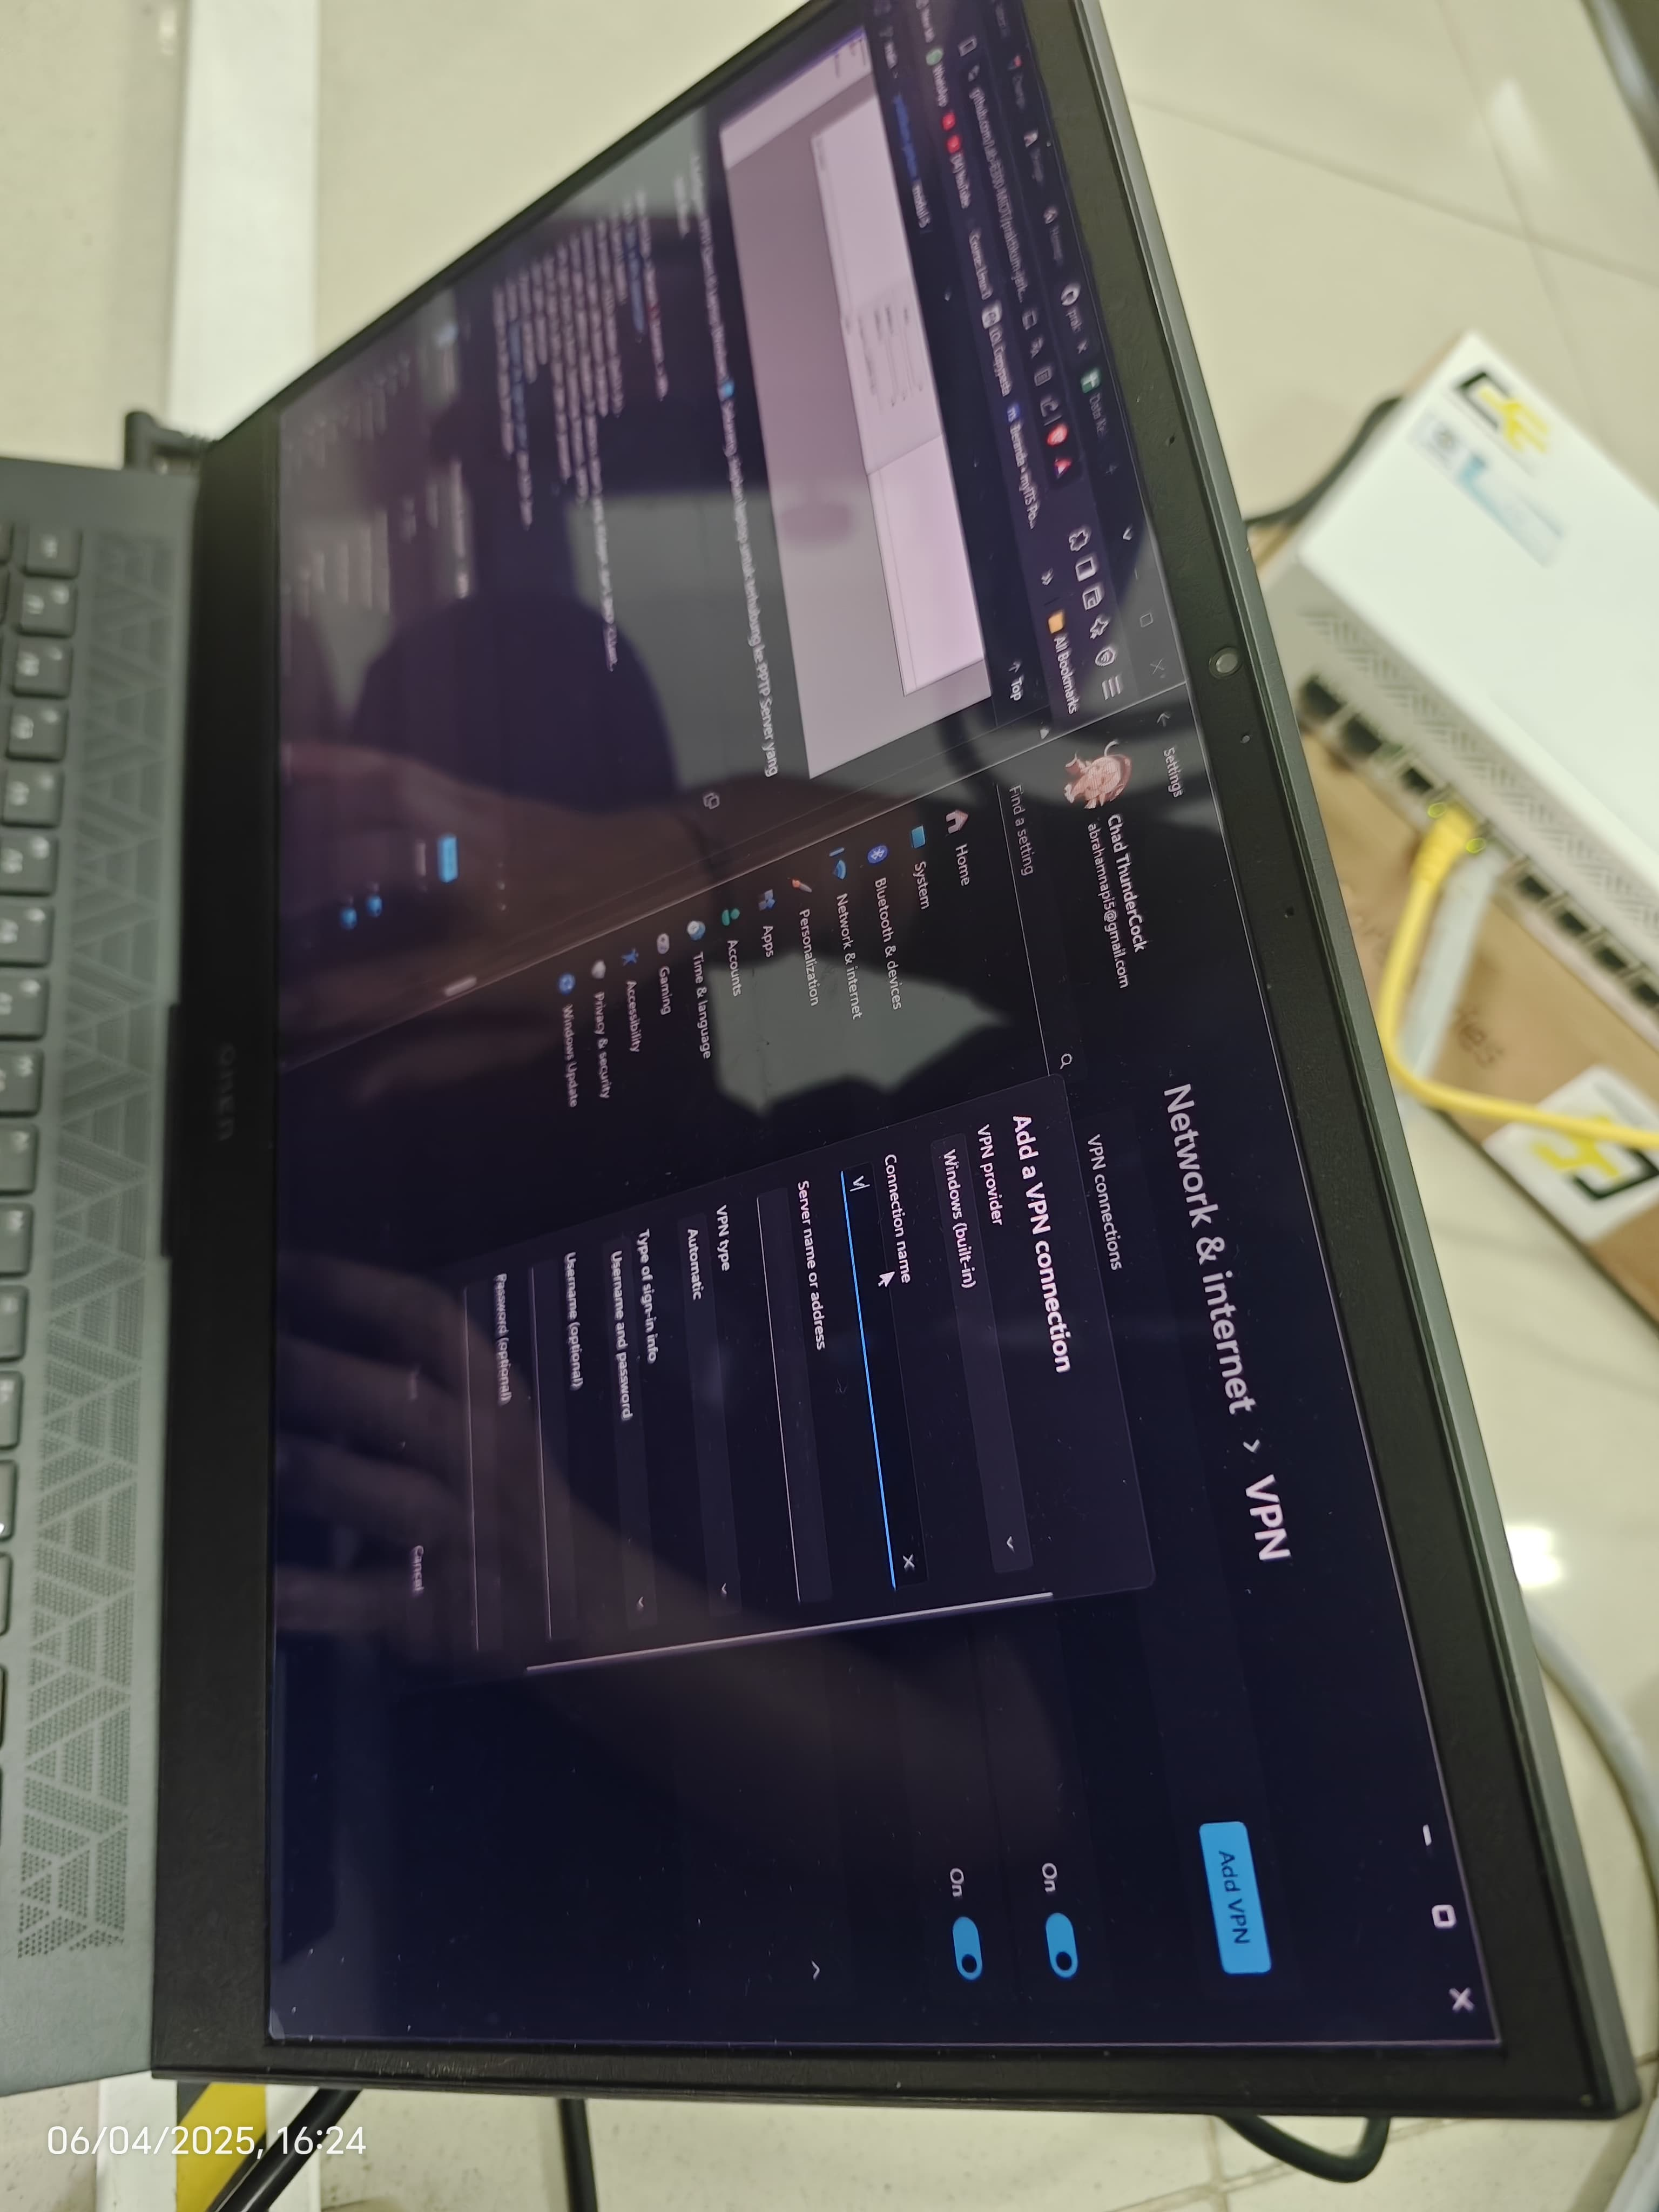
\includegraphics[width=0.7\textwidth]{P5/img/dokum.jpg}

